%
% Copyright © 2014 Sara Lelliott. All Rights Reserved.
%
\documentclass[letterpaper,12pt]{article}

%%%%%%%%%%%%%%%%%%%%%%%%%%%%%
%       LaTeX Packages      %
%%%%%%%%%%%%%%%%%%%%%%%%%%%%%
\usepackage{graphicx}
\usepackage{multirow}
\usepackage[section]{placeins}
\usepackage[affil-it]{authblk}
\usepackage{wrapfig}
\usepackage{tikz}
\usetikzlibrary{positioning,mindmap,shapes, decorations}
\usepackage{amsmath,amssymb}
\usepackage{bchart}
\usepackage{hyperref}
\usepackage{cleveref}
\usepackage{verbatimbox}
\usepackage[xindy,toc,acronym]{glossaries}
\makeglossaries
\usepackage[xindy]{imakeidx}
\makeindex
%%%%%%%%%%%%%%%%%%%%%%%%%%%%%

%%%%%%%%%%%%%%%%%%%%%%%%%%%%%%%%%%%%%%
% Tweak title page for multi-authors %
%%%%%%%%%%%%%%%%%%%%%%%%%%%%%%%%%%%%%%
\makeatletter
\def\@maketitle{%
  \newpage
  \null
  \vskip 2em%
  \begin{center}%
  \let \footnote \thanks
    {\Large\bfseries \@title \par}%
    \vskip 1.5em%
    {\normalsize
      \lineskip .5em%
      \begin{tabular}[t]{c}%
        \@author
      \end{tabular}\par}%
    \vskip 1em%
    {\normalsize \@date}%
  \end{center}%
  \par
  \vskip 1.5em}
\makeatother
%%%%%%%%%%%%%%%%%%%%%%%%%%%%%%%%%%%%%%

%%%%%%%%%
% Glossary %
%%%%%%%%%
\newglossaryentry{agile}
{
  name={Agile},
  description={The Agile developement model is one in which small incremental changes guide the final product to the customers ever changing requirements.}
}

\newacronym{mva}{MVA}{Model View Adapter}


%%%%%%%%%%%%%%%%%%
% Begin Document %
%%%%%%%%%%%%%%%%%%
\begin{document}
%.

%%%%%%%%%%%%%%%%%%%%%%%%%%%%% FIXME: emails..
% Primary document author %
\author{Sara Lelliott%
  \thanks{Electronic address: \href{mailto:slel0001@uni.sydney.edu.au}{slel0001@uni.sydney.edu.au}; Corresponding author}}
\affil{Department of IT, University of Sydney}
% Co-authors %
\author{Claire Lloyd-Prior%
  \thanks{Electronic address: \href{mailto:unikey@uni.sydney.edu.au}{unikey@uni.sydney.edu.au}}}
\affil{Department of IT, University of Sydney}
\author{Robert Schroder%
  \thanks{Electronic address: \href{mailto:unikey@uni.sydney.edu.au}{unikey@uni.sydney.edu.au}}}
\affil{Department of IT, University of Sydney}
\author{Callum Swain%
  \thanks{Electronic address: \href{mailto:unikey@uni.sydney.edu.au}{unikey@uni.sydney.edu.au}}}
\affil{Department of IT, University of Sydney}
\author{Michal Wahnon%
  \thanks{Electronic address: \href{mailto:unikey@uni.sydney.edu.au}{unikey@uni.sydney.edu.au}}}
\affil{Department of IT, University of Sydney}
\author{Eric%
  \thanks{Electronic address: \href{mailto:unikey@uni.sydney.edu.au}{unikey@uni.sydney.edu.au}}}
\affil{Department of IT, University of Sydney}
% Project Title %
\title{Website Project}
\date{Dated: \today}
%%%%%%%%%%%%%%%%%%%%%%%%%%%%%

%%%%%%%%%%%%%%%%%%%%%%%%%%%%%%%%%%%%%%%%%%%%%%%%%%%%%%%
% Construct Abstract/Title & Glossary of Figures here %
%%%%%%%%%%%%%%%%%%%%%%%%%%%%%%%%%%%%%%%%%%%%%%%%%%%%%%%
\maketitle
\begin{abstract}
  The purpose of this website is to educate the end user about the health risks of obesity and provide information on beneficial nutrition through interactive media such as a \acrfull{bmi} calculator, diet planner blog, quizzes and online games, whilst collecting quantitative data about the end user in order to help with further studies at the Charles Perkins Centre , while qualitative data is collected via surveys to help with the website's functionality.

The targeted end users are split up into easily defined groups so the website can collect data on specific age groups and also provide targeted information in a format relevant to those specifically targeted. The different end users are as following, "Parents and Kids", "Teens" and "Uni students".
\end{abstract}
\newpage
\listoffigures
\newpage
\tableofcontents
%%%%%%%%%%%%%%%%%%%%%%%%%%%%%%%%%%%%%%%%%%%%%%%%%%%%%%%

%%%%%%%%%%%%%
% Section 1 %
%%%%%%%%%%%%%
\section{Site Architecture}
% include figure 1
%
% Copyright © 2014 Sara Lelliott. All Rights Reserved.
%
\begin{figure}
  \centering
  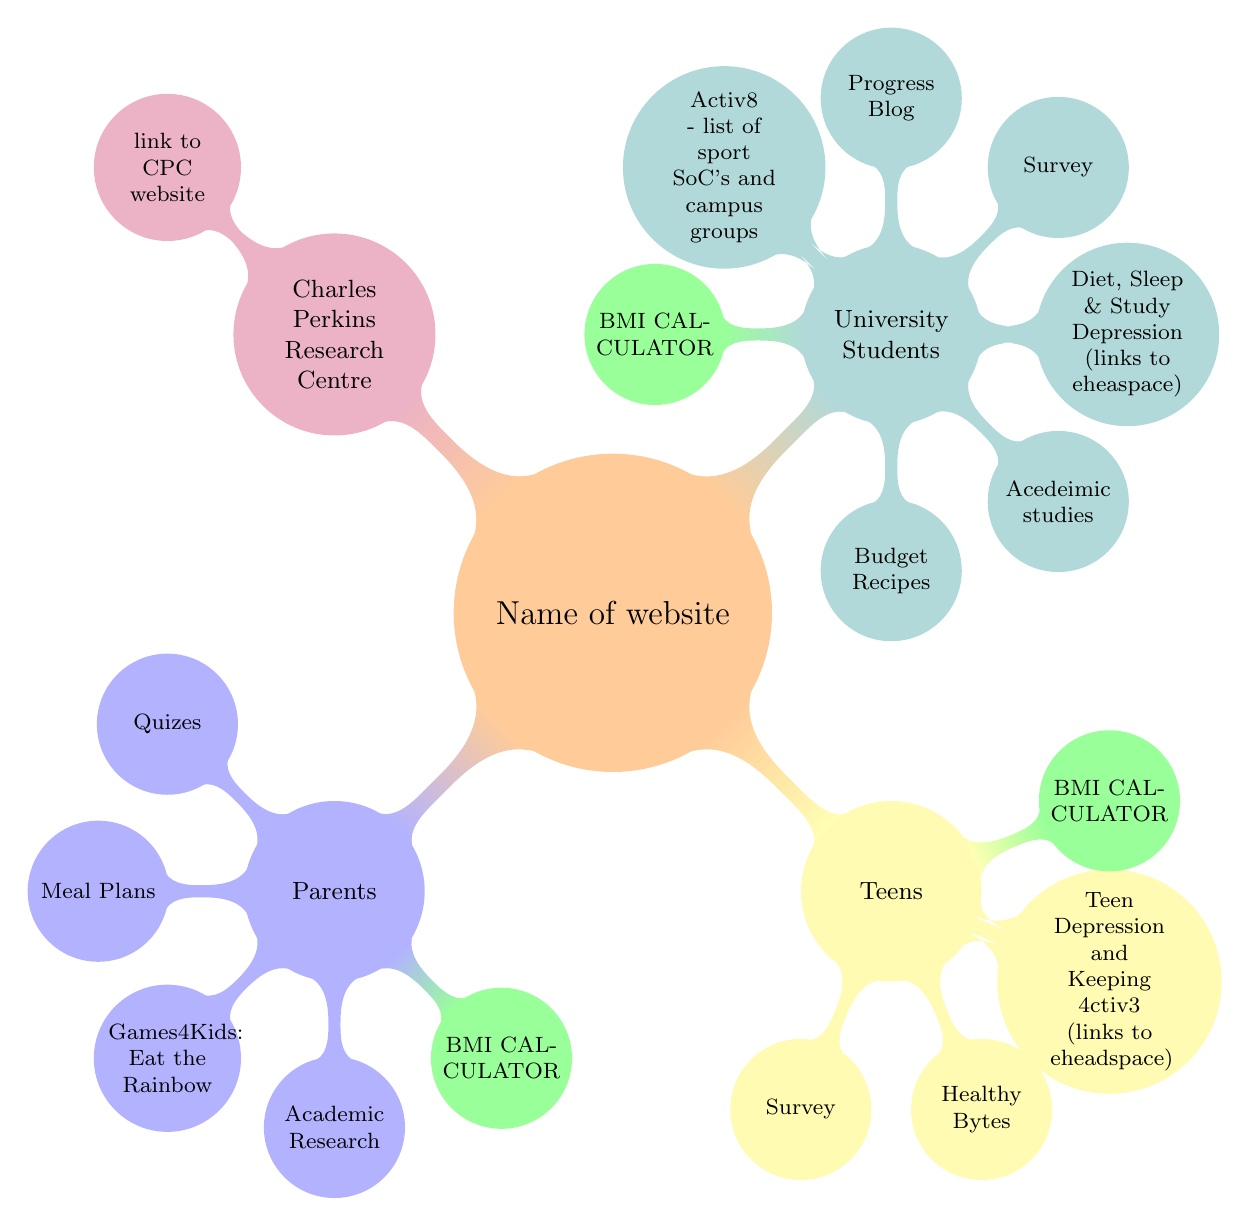
\begin{tikzpicture}[mindmap, grow cyclic, every node/.style=concept,
      concept color=orange!40,
      level 1/.append style={level distance=5cm,sibling angle=90},
      level 2/.append style={level distance=3cm,sibling angle=45},]
  %.
  \node{Name of website}
     child [concept color=blue!30] { node {Parents}
          child { node {Quizes}}
          child { node {Meal Plans}}
          child { node {Games4Kids: Eat the Rainbow}}
          child { node {Academic  Research}}
          child [concept color=green!40] { node {BMI CALCULATOR}}
      }
      child [concept color=yellow!30] { node {Teens}
          child { node {Survey}}
          child { node {Healthy Bytes}}
          child { node {Teen Depression and Keeping 4ctiv3 (links to eheadspace)}}
          child [concept color=green!40] { node {BMI CALCULATOR}}
      }
      child [concept color=teal!30] { node {University Students}
          child { node {Budget Recipes}}
          child { node {Acedeimic studies}}
          child { node {Diet, Sleep \& Study Depression (links to eheaspace)}}
          child { node {Survey}}
          child { node {Progress Blog}}
          child { node {Activ8 - list of sport SoC's and campus groups}}
          child [concept color=green!40] { node {BMI CALCULATOR}}
      }
      child [concept color=purple!30] { node {Charles Perkins Research Centre}
          child { node {link to CPC website}}
      };
  %.
  \end{tikzpicture}
  \caption{Sub-domain Hierarchy}
  \label{fig:subdomain-hierarchy}
\end{figure}

.
% include site_map.txt
%
% Copyright © 2014 Sara Lelliott. All Rights Reserved.
%
\begin{verbbox}

                                            +--------+ +------+   +--------+
                                            |register| |log in|   |site map|
                                            +--------+ +------+   +--------+



                                +-------------+
                                |contact us/  |
                                | credits     |
  +--------------------+        +---+---------+
  |                    |            |
  | home               +------------+--------------+
  |                    | +----------+-----+   +----+-----------+
  |                    | |about us/mission|   |CHARLES PERKINS |
  +-+-+------------+---+ | statement      |   | SITE           |
    | |            |     +-----+----------+   +----------------+
    | |            |
    | |            |
    | |   +--------v------+       +---------------+     +--------------+
    | |   |parents        +-------> BMI           +-----+ kids         |
    | |   +-----+---------+       +----+----------+     +----+---------+
    | |         |                      |                     |
    | |         |                      |                     |
    | |   +-----v--------+             |                     |
    | |   |meal plans    |       +-----v---------+    +------v-----------+
    | |   +-----+--------+       |quiz           |    | games            |
    | |         |                +---------------+    +------------------+
    | |   +-----+--------+
    | |   |blog          |
    | |   +--------------+
    | |
    | |
    | |
    | |
    | |
    | |  +--------------+      +----------+
    | +--+ teens        +------+ quizes   |
    |    +--------+-----+      +----------+
    |             |
    |             |           +--------------+
    |             +-----------+ BMI          |
    |                         | CALCULATOR   |
    |                         +--------------+
    |
    |
    |    +--------------+      +----------+
    +----+ uni students +------+ blog     |
         +---+----------+      +----------+
             |
             |           +--------------+
             +-----------+ BMI          |
                         | CALCULATOR   |
                         +--------------+

\end{verbbox}
\resizebox{0.95\textwidth}{!}{\theverbbox}


%% .. %%
\section{End user types and their page layouts}
\subsection{Parents and Kids}

This page will consist of information on what childhood obesity is and contain statistics on how many Australian children are affected by this disease and other associated health risks. There will be a link to a \acrfull{bmi} calculator, quizzes that parents can do with their child, an interactive game called "Eat the Rainbow", which encourages healthy food choices and pictures of physical activities that can be fun to encourage kids to play outside and develop positive habits to help them in later years. There will also be Information on developing healthy meal plans and recipes that cater to gluten free, dairy free, halal, kosher and vegan diets and a survey to ascertain qualitative data about the website.

%% .. %%
\subsection{Teens}

The Teen page will consist of photos of young people having fun out doors as well as fun indoors. There will also be links to "4ctiv3" a page of information on teen depression, connected to hormones and sleep patterns and not enough physical activity with links to eheadspace if further help is needed. There will be a links to a survey page to help collect data from the end user in order to verify whether this page is helpful and reaching the demographic, a function that could be added as an incentive, every x amount survey the user does they receive a \$10 Coles Myer gift voucher. There will be also a page called "Healthy Bytes" which has recipes for healthy snacks and exercises to do between online gaming sessions as poor eating habits can be developed at this time. There will also be a link to the \acrshort{bmi} calculator.

%% .. %%
\subsection{University Students}

The main body of the University Student page will contain photos of young people outside at the beach, gym and studying. There will be information about why ample sleep and a balance diet is important to maintain health while studying. There will be a link called "Activat8" which will be a list of health/fittness SoCs and campus groups. There will be a link to a customisable progress blog where students can record there meals and cheat days and organise their diet and excercise. There will also be a link budget recipes so poor students won't have to resort to junk food to survive and a link to relevant acedemic studies on obesity and young adults. There will be a link to a survey to improve site functionality and \acrshort{bmi} calculator.

%% .. %%
\section{Other Page Descriptions linked from the Main page}

\subsection{The Charles Perkins Centre}

The Charles Perkins Centre page will contain a brief description of who Charles Perkins was and what research is done there, also ther will be a link to the Charles Perkin's Centre website.

\subsection{Mission Statement} 

A page where we outline our core values and what we wish to achieve with this website and another list of useful links and related sources.

\subsection{About us}

About us will list the contributors to this website and contact.

%% .. %%
\section{Design philosphy of the Website}

\subsection{Development Life Cycle}

We propose that we incorperate A/B Testing in both \Gls{agile} and Iterative design philosophies as both have advantages and disadvantages and will add dynamism to the project. Version control will assist in running concurent concepts. 

\subsubsection{Agile Testing}

\Gls{agile} testing has a time to market advantage. So when the project is in it's up time phase, beta testing can commence with a sample of endusers.

\subsubsection{Iterative Testing}

This style of testing can be expensive for a life time of a project so it was only used in the conceptualisation phase.

\subsubsection{Model-View-Adapter}

The interaction of user data and server software state is often a attack vector
as to nefariously miss-configure the server or simply to take advantage of
miss-configuration of the intended user by an adversary. We propose a novel
isolation of the user data state and view from a known \emph{secure by default}
configuration.

The user session data is dealt is by means of a \emph{client-server}
model in the context of \gls{restful} internet applications, in which
the \emph{user interface}, \emph{programatic logic}
and \emph{storage} are \textbf{separated} out as
independent modular software components. We fix here the terminology of,
\emph{presentation}, \emph{logic} and \emph{data} to the respective
components.

% Include the MVC/MVA Model diagram %
%
% Copyright © 2014 Sara Lelliott. All Rights Reserved.
%
\begin{figure}[ht!]
  \begin{center}
    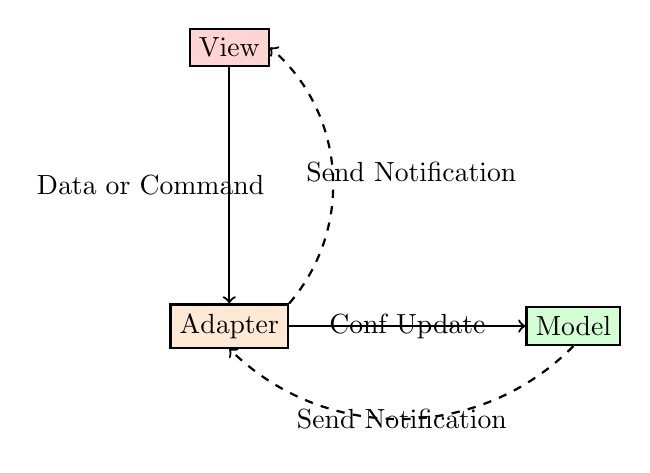
\begin{tikzpicture}[thick]
      % View
      \node[rectangle,draw,fill=red!17] (view) {View};
      % Adapter
      \node[rectangle,draw,below=3.0cm of view,fill=orange!17] (adapter) {Adapter};
      % Model
      \node[rectangle,draw,right=3.0cm of adapter,fill=green!17] (model) {Model};
      % interactions..
      \draw[->] (view.south) -- node[left of=adapter] {Data or Command} (adapter.north);
      \draw[->] (adapter.east) -- node {Conf Update} (model.west);
      % notification
      \draw[->,dashed] (model.south) to [bend left=45] node {Send Notification} (adapter.south);
      \draw[->,dashed] (adapter.north east) to [bend right=45] node[right of=data] {Send Notification} (view.east);
    \end{tikzpicture}
    \caption{Model-View-Adapter Architecture}
    \label{fig:mva-arch}
  \end{center}
\end{figure}

This~\cref{fig:mva-arch} three-tier design is in fact the \acrfull{mva} architectural pattern. In contrast to the Model View Controller (MVC)
pattern, the \acrshort{mva} pattern does not allow the \emph{view} component to interact
directly with the \emph{data} component instead requests are mediated via the
\emph{adapter} component.

The configuration state modifications expressed in the \emph{view} component
are mediated by the \emph{adapter} components logic and packed up for storage
in the \emph{data} component. The \emph{data} component implements the
interaction with a database to store modifications to a user session.

%% .. %%
\section{Site Layout}

Primary~\cref{fig:layout-mainpage} (Site A.) site.
\begin{figure}[ht!]
  \centering
  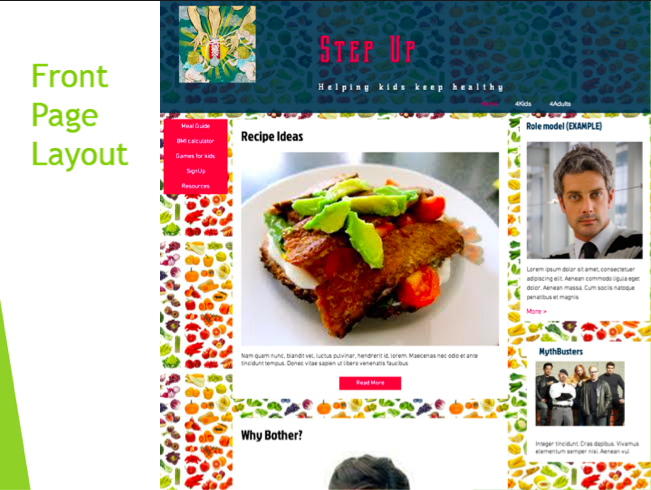
\includegraphics[width=0.9\textwidth]{assets/jpg/layout_mainpage}
  \caption{Layout of main (A.) page}
  \label{fig:layout-mainpage}
\end{figure}
\FloatBarrier

%% .. %%
\section{Design Comparisons}

%% FIXME: Use Excel plugin to export these later and include them
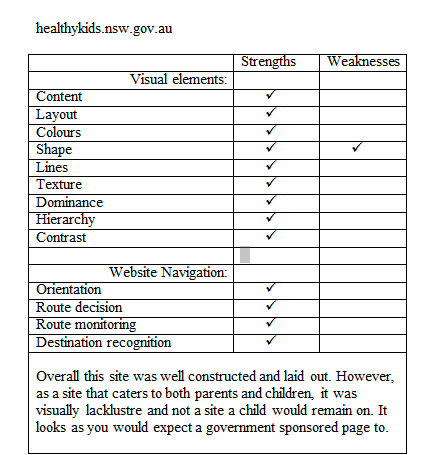
\includegraphics[width=0.9\textwidth]{assets/jpg/tab1}

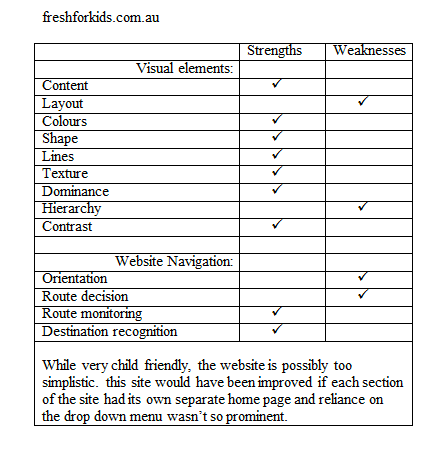
\includegraphics[width=0.9\textwidth]{assets/jpg/tab2}

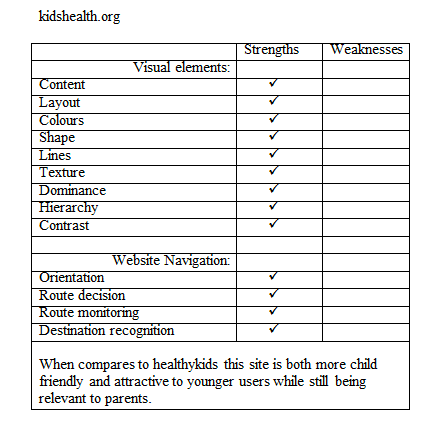
\includegraphics[width=0.9\textwidth]{assets/jpg/tab3}
%%%%

Other sites found are seen here~\cref{fig:othersites}
%\begin{table}[ht]
 % \centering
 % \begin{tabular}{cc}
 %   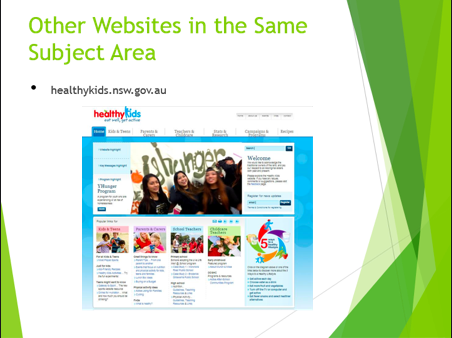
\includegraphics[scale=1]{assets/jpg/othersite_1}
 %   &
\includegraphics[scale=1]{assets/jpg/othersite_2}\\
 %   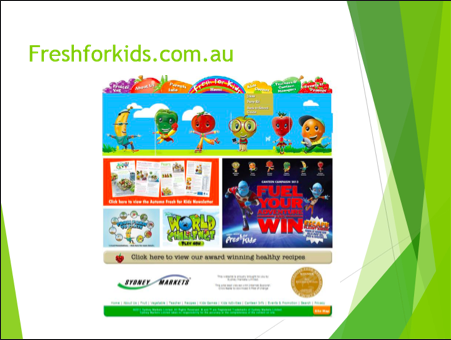
\includegraphics[scale=1]{assets/jpg/othersite_3}
 %   &..\\
 % \end{tabular}
 % \caption{Other sites}
 % \label{tab:othersites}
%\end{table}

\begin{figure}[ht!]
  \centering
  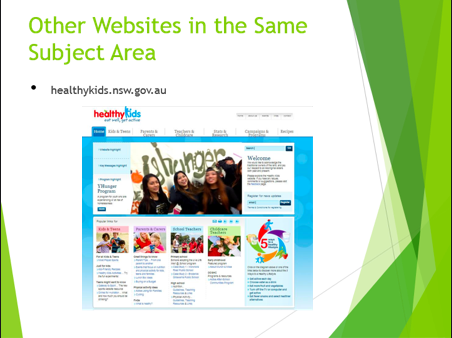
\includegraphics[width=0.9\textwidth]{assets/jpg/othersite_1}
  \caption{Other sites 1}
  \label{fig:othersites}
\end{figure}
\FloatBarrier

\begin{figure}[ht!]
  \centering
  
\includegraphics[width=0.9\textwidth]{assets/jpg/othersite_2}
  \caption{Other sites 2}
  \label{fig:othersites-2}
\end{figure}
\FloatBarrier

\begin{figure}[ht!]
  \centering
  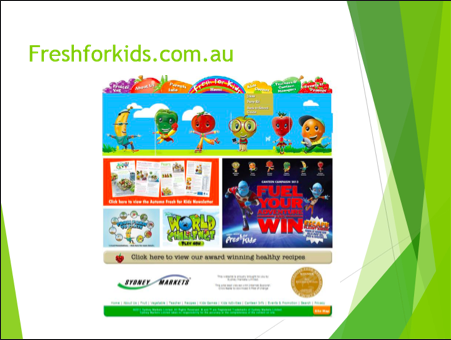
\includegraphics[width=0.9\textwidth]{assets/jpg/othersite_3}
  \caption{Other sites 3}
  \label{fig:othersites-3}
\end{figure}
\FloatBarrier

%% .. %%
\section{Domain name}

\url{Stepup.org} is the domain the group chose. We have done this to encourage the Enduser to rise to the challange and fight obesiety through daily excercise and healthy eating.

%% .. %%
\section{Story Board}

\begin{figure}[ht!]
  \centering
  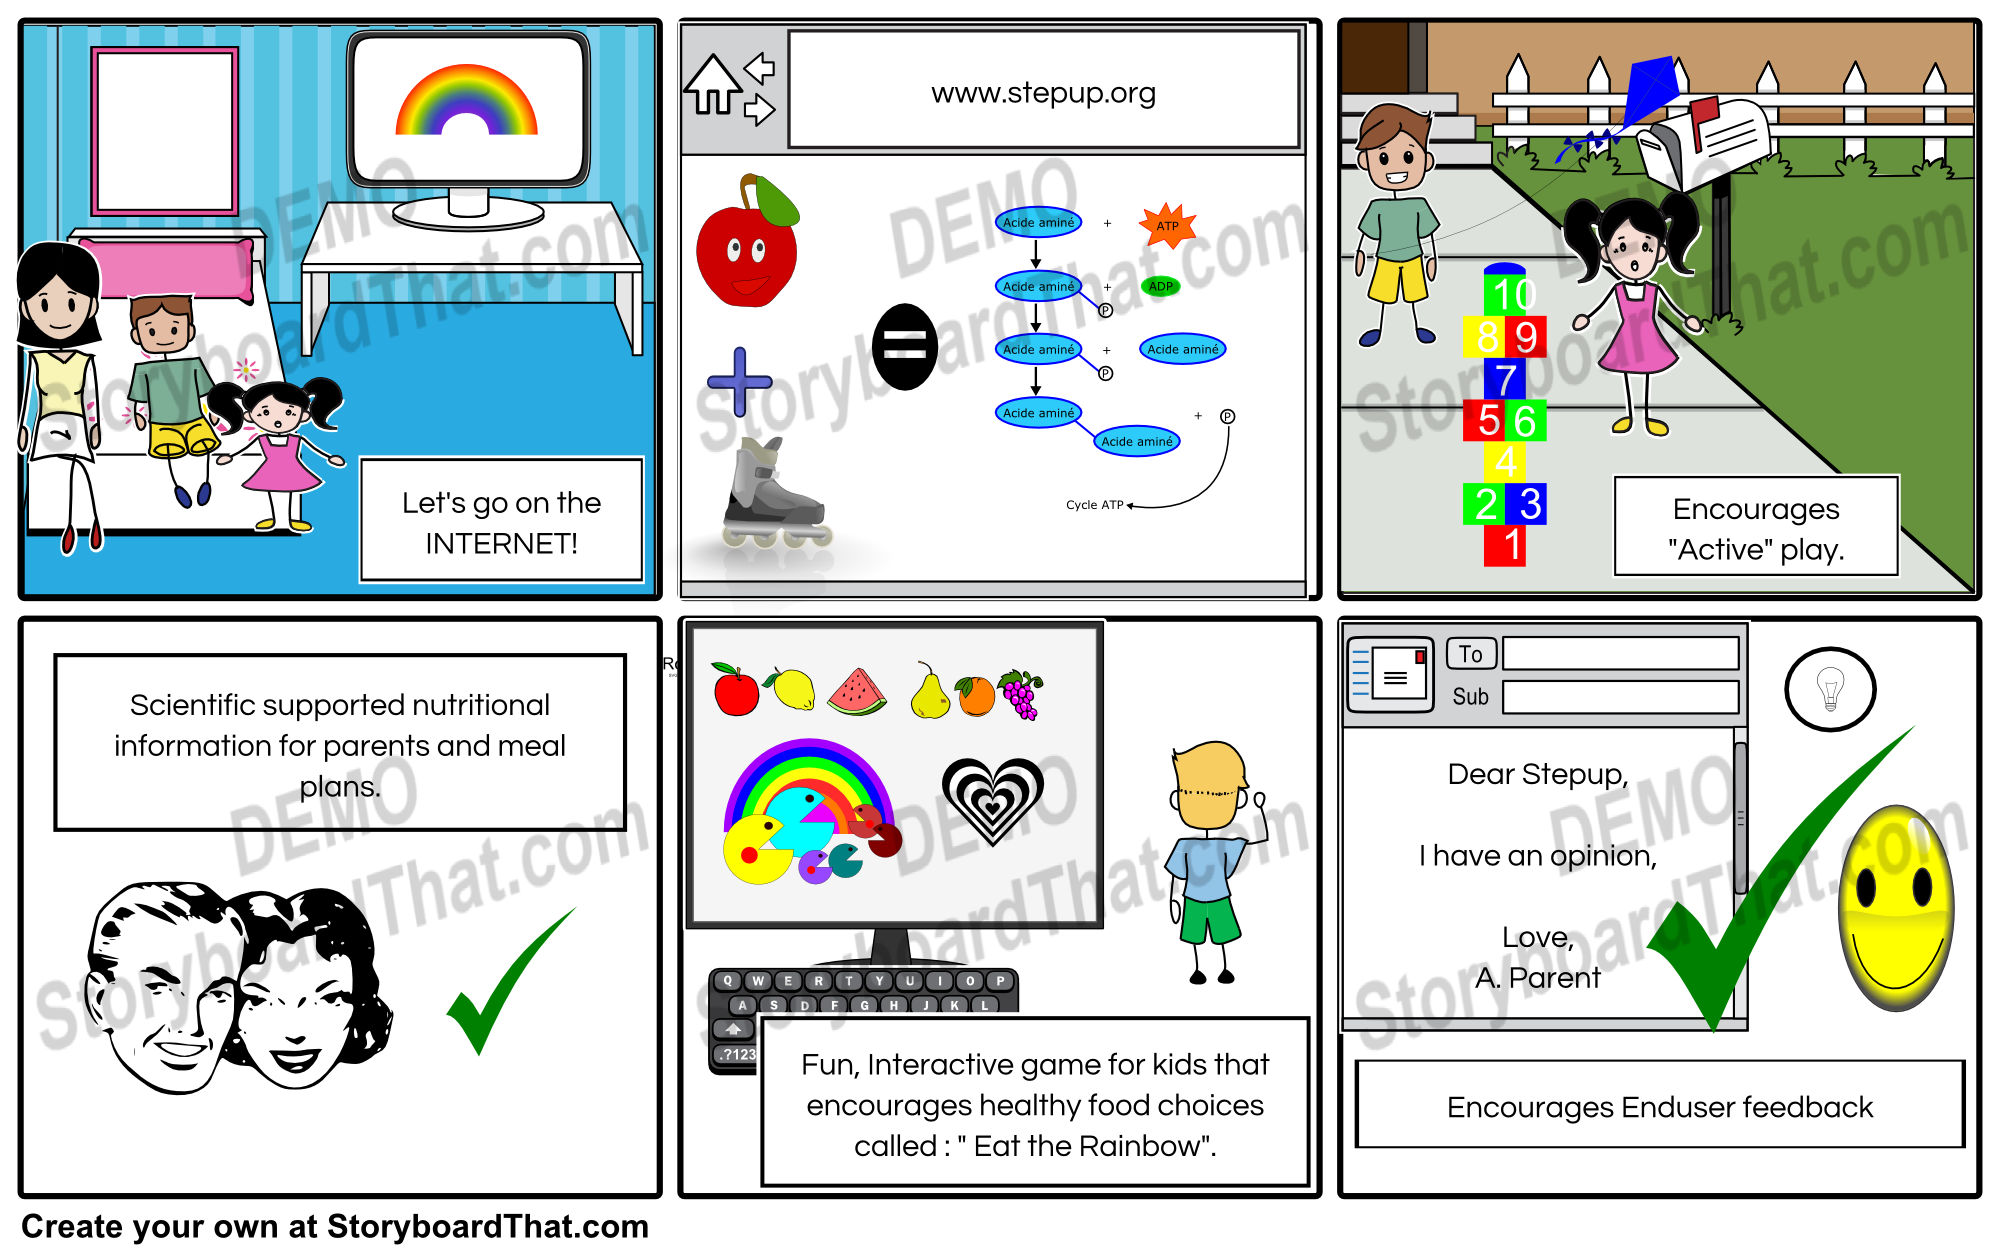
\includegraphics[width=0.9\textwidth]{assets/jpg/parent_and_children_experience}
  \caption{Storyboard of End User Experience: Parent and Child}
  \label{fig:parent-and-children-experience}
\end{figure}
\FloatBarrier
\begin{figure}[ht!]
  \centering
  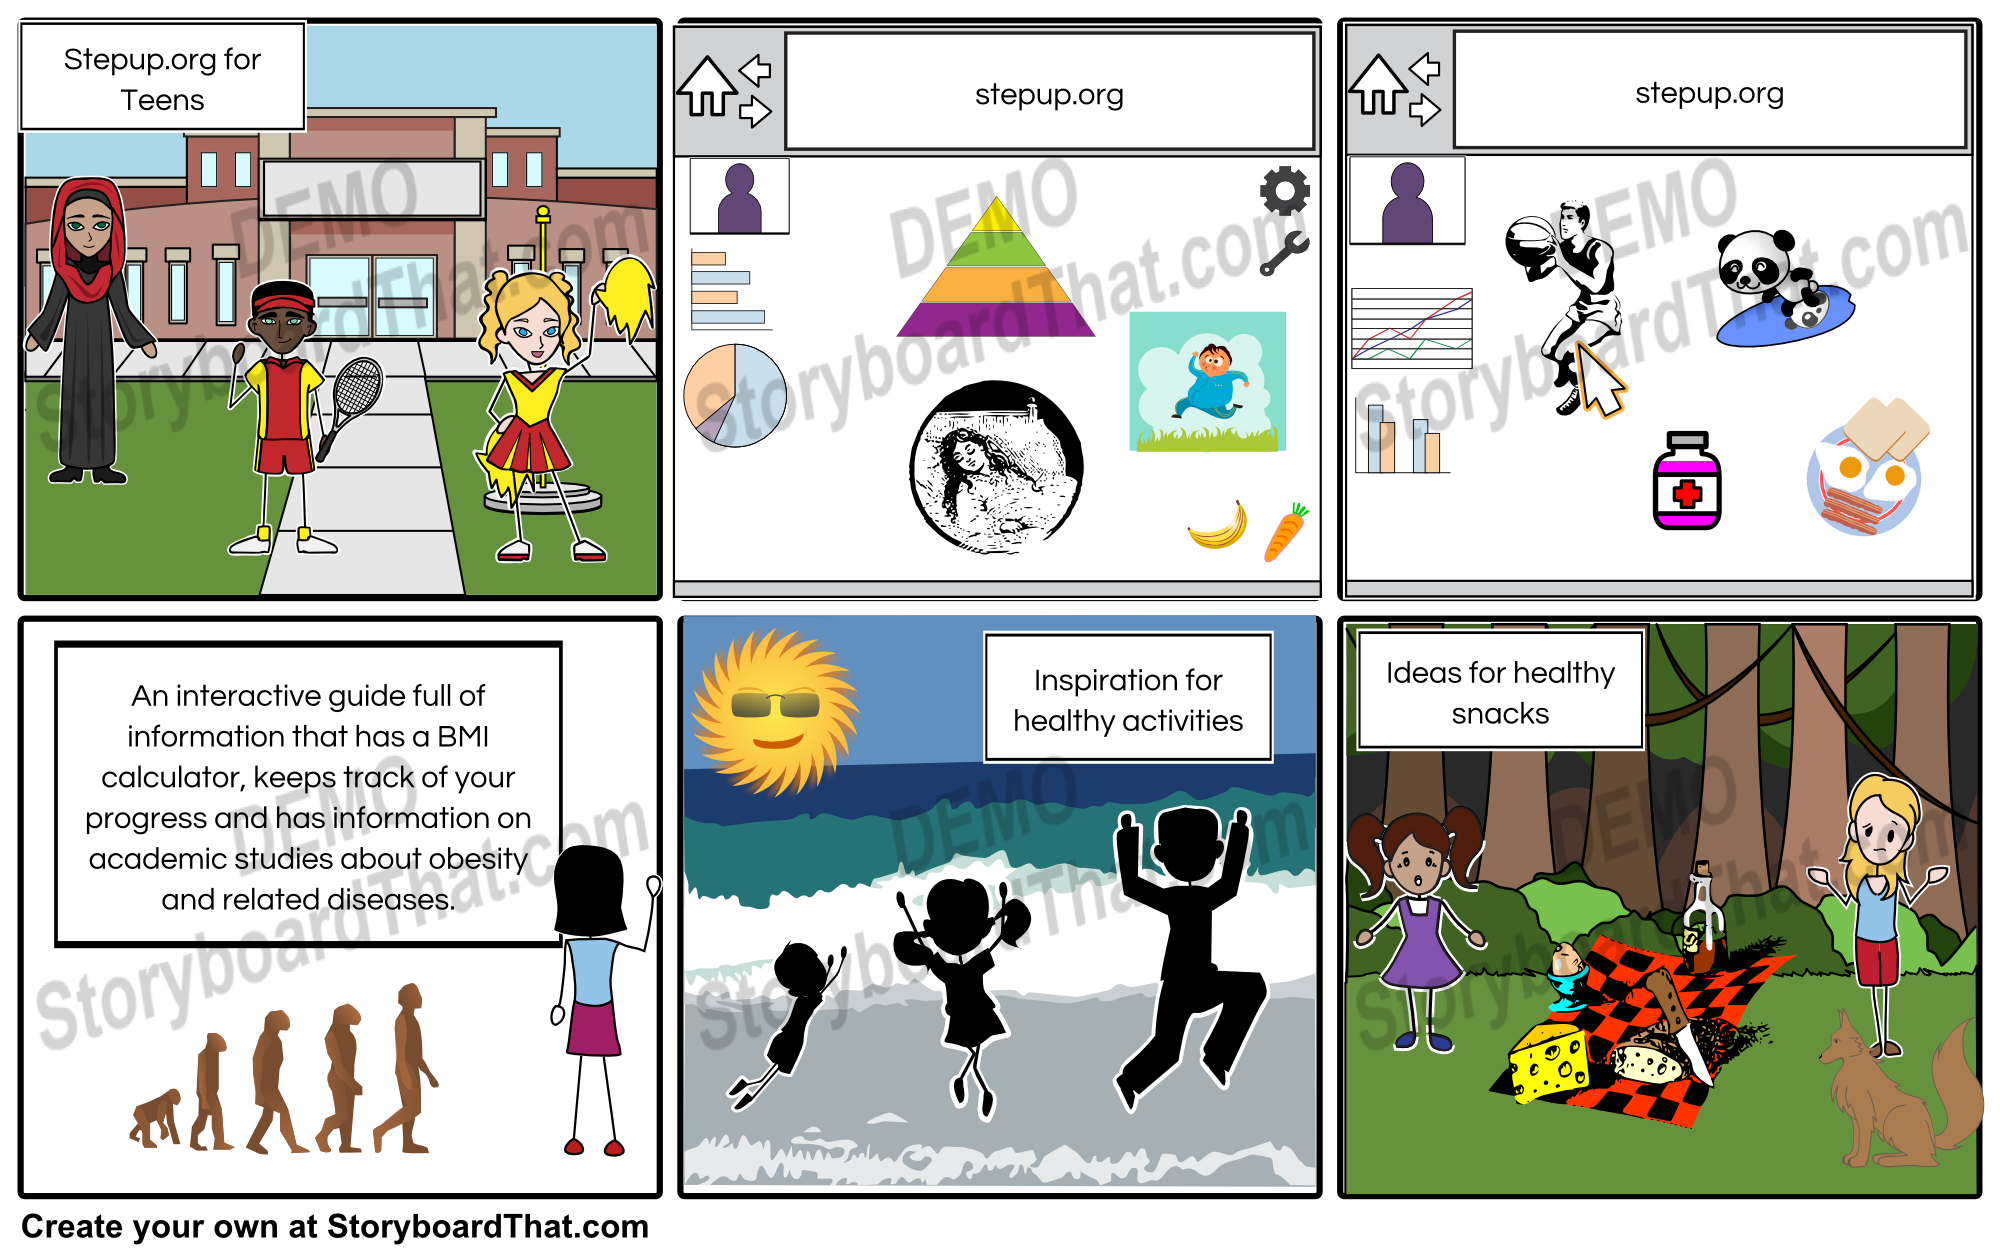
\includegraphics[width=0.9\textwidth]{assets/jpg/stepup_com_scenario_2}
  \caption{Storyboard of End User Experience: \url{stepup.com} scenario}
  \label{fig:stepup-com-scenario-2}
\end{figure}
\FloatBarrier

%% .. %%
\section{Survey Questions and Analysis}

\begin{figure}[ht!]
  \centering
  \begin{bchart}[step=15,max=45,width=12cm]
    \bcbar[label=Unfamiliar,value=3]{3}
    \bcbar[label=Somewhat Fair,value=37,color=red]{37}
    \bcbar[label=Comfortable,value=21]{21}
    \bcbar[label=Very Good,value=35]{35}
    \bcbar[label=Exellent,value=1]{1}
  \end{bchart}
  \caption{Heathy Eating Paterns}
  \label{tab:heating-patterns}
\end{figure}

%% .. %%
\section{Questions for other Teams}

\subsection{Security}

\begin{itemize}
  \item
What security messures will you use to santise user input (protect client data from malicious code being entered into the form eg. escape characters)?
  \item
Does the site have a vaild \gls{ssl} certificate?
\end{itemize}

\subsection{Search Engine Indexing}

What about \gls{sco} considerations?

% Define box and box title style
\tikzstyle{mybox} = [
    draw=red,
    fill=blue!20,
    very thick,
    rectangle,
    rounded corners,
    inner sep=10pt,
    inner ysep=20pt
]
\tikzstyle{fancytitle} =[fill=red, text=white]

\begin{figure}
  \centering
\begin{tikzpicture}
    \node [mybox] (box){
        \begin{minipage}{0.9\textwidth}
            $\underbrace{\text{http}}_{\text{protocol}}
\text{://}
\underbrace{
\overbrace{\text{stepup}}^\text{2\textsuperscript{nd} level domain}
\text{.}
\overbrace{\text{com}}^\text{TLD}
}_\text{hostname}
\underbrace{\text{/why-eat-well/}}_\text{path}
\text{\#}
\underbrace{\text{eatting\_is\_fun}}_\text{Fragment identifier}$
        \end{minipage}
    };
    \node[fancytitle, right=10pt] at (box.north west) {The URL};
\end{tikzpicture}
  \caption{The structure of a \acrfull{url}.}
\end{figure}

\subsection{Research}

What qualitive data have you gathered to test whether methods implemented on the website will ensue the return of the end user?

\subsection {Design}

In regards to potential flaws in design philosphy, what actions have you taken to compensate for these flaws?

%%%%%%%%%%
% Appendix %
%%%%%%%%%%
\appendix
\printindex
\glossarystyle{listhypergroup}
\printglossaries

%%%%%%%%%%%%%%%%
% End Document %
%%%%%%%%%%%%%%%%
\end{document}
%.